\documentclass[18pt]{beamer}
\usepackage[utf8]{inputenc} % for the umlauts
\usepackage{subfigure}

\beamertemplatenavigationsymbolsempty
%% SLIDE FORMAT

% use 'beamerthemekit' for standard 4:3 ratio
% for widescreen slides (16:9), use 'beamerthemekitwide'

\usepackage{templates/beamerthemekit}
% \usepackage{templates/beamerthemekitwide}

\setcounter{tocdepth}{1}

%% TITLE PICTURE

% if a custom picture is to be used on the title page, copy it into the 'logos'
% directory, in the line below, replace 'mypicture' with the 
% filename (without extension) and uncomment the following line
% (picture proportions: 63 : 20 for standard, 169 : 40 for wide
% *.eps format if you use latex+dvips+ps2pdf, 
% *.jpg/*.png/*.pdf if you use pdflatex)

%\titleimage{mypicture}

%% TikZ INTEGRATION

% use these packages for PCM symbols and UML classes
% \usepackage{templates/tikzkit}
% \usepackage{templates/tikzuml}

% the presentation starts here

\usepackage{mathabx}
\usepackage{picture}
\usepackage{csquotes}
\usepackage[absolute,overlay]{textpos}
%\usepackage[texcoord,grid,gridunit=mm,gridcolor=red, subgridcolor=green]{eso-pic}
\setbeamercovered{invisible}
\setbeamertemplate{caption}{\raggedright\insertcaption\par}

\title[SWT1]{Softwaretechnik 1 - 5. Tutorium}
\subtitle{Tutorium 17}
\author{Felix Bachmann}
\date{09.07.2019}

\institute{KIT - Institut für Programmstrukturen und Datenorganisation (IPD)}

\begin{document}
% change the following line to "ngerman" for German style date and logos
\selectlanguage{ngerman}
	
%title page
\begin{frame}
\titlepage
\end{frame}

\begin{frame}
\tableofcontents
\end{frame}


\section{Orga}
	\begin{frame}{Demokratie ist 'ne super Sache}
		\begin{itemize}
			\item wir können das Studierendenparlament und FachschaftssprecherInnen wählen
			\item noch die gesamte Woche
			\item bei der Mensa, AKK, oder Fachschaft (egal wo)
			\item es gibt Kekse!
			\item weitere Informationen
			\begin{itemize}
				\item \url{https://wahl.asta.kit.edu/Wahl19/stupaomat/stupaomat.html}
				\item \url{https://wahl.asta.kit.edu/}
			\end{itemize}
		\end{itemize}
	\end{frame}

	\begin{frame}{Allgemeines}
		\begin{alertblock}{Nächstes Mal ist schon letztes Tutorium} 
		\begin{itemize}
			\item geplant: grobe Wiederholung + viele Klausuraufgaben \pause
			\item ansonsten irgendwelche Wünsche?
			\begin{itemize}
				\item etwas bestimmtes wiederholen?
				\item nochmal irgendwas erklären?
				\item Beispiel für XY?
				\item falls euch noch was einfällt, schreibt mir eine Mail
				\linebreak $\implies$ felix.bachmann@ewetel.net
			\end{itemize}
		\end{itemize}
		\end{alertblock}
	\end{frame}

	\begin{frame}{5. Übungsblatt Statistik}
		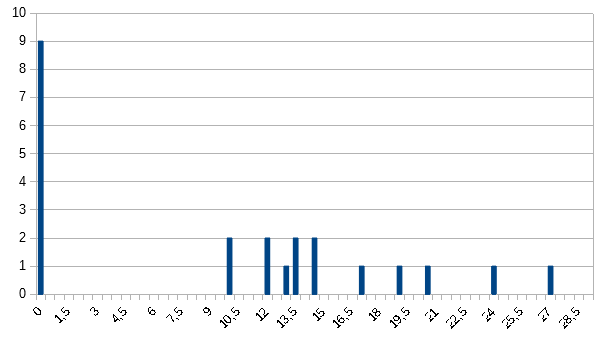
\includegraphics[scale=0.7]{./pics/tut5/statistics-ub5.png}
	\end{frame}

	\begin{frame}{Häufige Fehler}
		\begin{block}{Allgemein}
			\begin{itemize}
				\item (mal wieder\dots) CheckStyle und JavaDoc
			\end{itemize}
		\end{block}
	\end{frame}

	\begin{frame}{Häufige Fehler}
		\begin{block}{Aufgabe 1: MVC als Schichtenarchitektur}
			\begin{itemize}
				\item Methoden/Attribute fehlten
				\begin{itemize}
					\item Semantik? 
					\item Beobachter, Klick/Registrierkomponenten, etc.?
				\end{itemize}
				\pause
				\item Beobachter Model $\leftrightarrow$ View nicht modelliert \pause
				\item uses-Beziehung 
				\begin{itemize}
					\item fehlte
					\item falsche Syntax
					\item Pfeile zwischen Paketen sind zu offensichtlich
				\end{itemize}
			\end{itemize}
		\end{block}
	\end{frame}

	\begin{frame}{Häufige Fehler}
		\begin{block}{Aufgabe 2: Entwurfsmuster \texttt{CacheProvider}}
			\begin{itemize}
				\item falsches Muster
				\item häufig: Strategie oder Fabrikmethode \pause
				\item Strategie ist oft der \enquote{easy way out}
				\begin{itemize}
					\item viele (wenn nicht alle) EMs nutzen Strategie
					\item dafür reicht ja quasi schon eine Schnittstelle \pause
					\item daher: erst größere Muster \enquote{um Strategie herum} suchen
					\item Strategie bei solchen Fragen nur antworten, wenn ihr gar nix findet
				\end{itemize}
			\end{itemize}
		\end{block}
		\pause 
		\begin{block}{Aufgabe 3: Entwurfsmuster impl. (Iterator, Besucher)}
			\begin{itemize}
				\item Prinzip: Iterator benutzt Visitor um nächstes Element herauszufinden
				\item Zusammenhang war manchmal nicht ganz klar
			\end{itemize}
		\end{block}
	\end{frame}

	\begin{frame}{Häufige Fehler}
		\begin{block}{Aufgabe 4: Code $\rightarrow$ Klassendiagramm}
			\begin{itemize}
				\item wie in VL-Folien
				\begin{itemize}
					\item Map=qualifizierte Assoziation
					\begin{itemize}
						\item Achtung, Multiplizität \underline{pro Qualifizierer}
					\end{itemize}
					\item Set=\texttt{\{unique\}}
				\end{itemize}
				\pause
				\item Attribute nicht mehr hinschreiben, wenn bereits die Assoziation da steht
			\end{itemize}
		\end{block}
		\pause
		\begin{block}{Aufgabe 5: Zustandsmuster(Kaffeemaschine) impl.}
			\begin{itemize}
				\item explizite, ausgelagerte Zustandshaltung sollte verwendet werden
				\begin{itemize}
					\item einfach Vorlesungsfolien \enquote{nachimplementieren}
				\end{itemize}
				\item Reminder: im UML-Zustandsdiagramm tun nicht definierte Übergänge nichts
				\begin{itemize}
					\item wie in VL kann es aber sinnvoll sein Exceptions zu werfen
					\item abhängig vom Anwendungsfall, hier war beides ok
				\end{itemize}
			\end{itemize}
		\end{block}
	\end{frame}

	\begin{frame}{Häufige Fehler}
		\begin{block}{Aufgabe 6: \texttt{git merge} vs \texttt{git rebase}}
			\begin{itemize}
				\item beim rebasen zwei Probleme
				\begin{itemize}
					\item feature an master \enquote{ran-gerebased}
					\begin{itemize}
						\item Kollegen arbeiten auf altem master ohne die feature commits
					\end{itemize}
					\pause
					\item master an feature \enquote{ran-gerebased}
					\begin{itemize}
						\item zwei master-Branches! 
						\item autsch
					\end{itemize}
				\end{itemize}
			\end{itemize}
		\end{block}
	\end{frame}

	\begin{frame}{Jetzt letztes Übungsblatt..}
		\begin{huge}
			Falls ihr noch Punkte braucht, gebt ab!
		\end{huge}
\end{frame}

\section{Überblick}
	\subsection{Überblick}
	\begin{frame}
		\frametitle{Überblick}
		\centering \huge Wo sind wir?
	\end{frame}
	
	
\section{Parallelität}
	
	\begin{frame}{Programm vs. Prozess vs. Thread}
		\begin{itemize}
			\item Programm = ausführbare Datei
			\item Prozess = Programm in Ausführung
			\item Thread = Ausführungseinheit innerhalb eines Prozesses
		\end{itemize}
	\end{frame}
	
	\begin{frame}
		\frametitle{Grundlagen}
		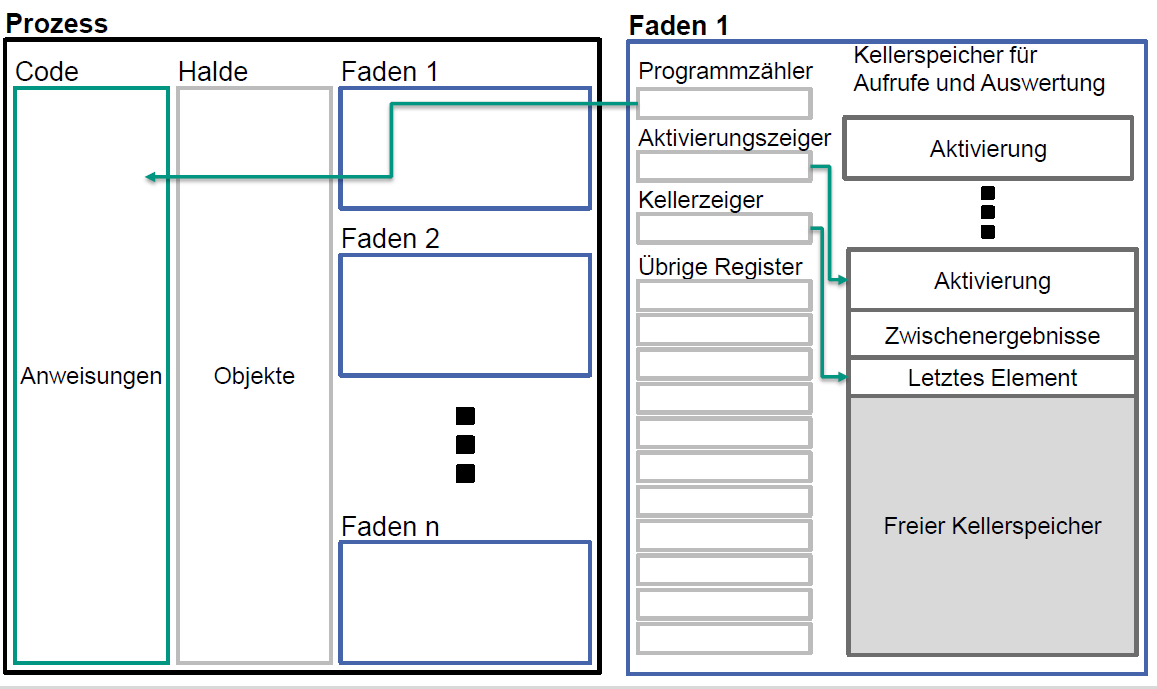
\includegraphics[scale=0.34]{./pics/tut5/proc-thr.png}
	\end{frame}

	\begin{frame}
		\frametitle{Grundlagen}
		\begin{itemize}
			\item Prozess = Programm in Ausführung \pause
			\item jeder Prozess hat eigenen Adressraum (= Speicherbereich im Arbeitsspeicher) \pause
			\item jeder Prozess hat mindestens einen Thread \pause
			\item Threads existieren innerhalb eines Prozesses \pause 
			\begin{itemize}
				\item Threads haben den gleichen Heap und Code \pause 
					\linebreak $\implies$ alle Threads innerhalb eines Prozesses arbeiten mit denselben globalen Variablen und demselben Code \pause 
				\item Threads haben eigene Stacks und Befehlszeiger (Programmzähler) \pause 
					\linebreak $\implies$ Threads haben eigene lokale Variablen und können beliebigen Code des Prozesses ausführen
			\end{itemize}
		\end{itemize}
	\end{frame}
	
	
	\begin{frame}
		\frametitle{Motivation}
		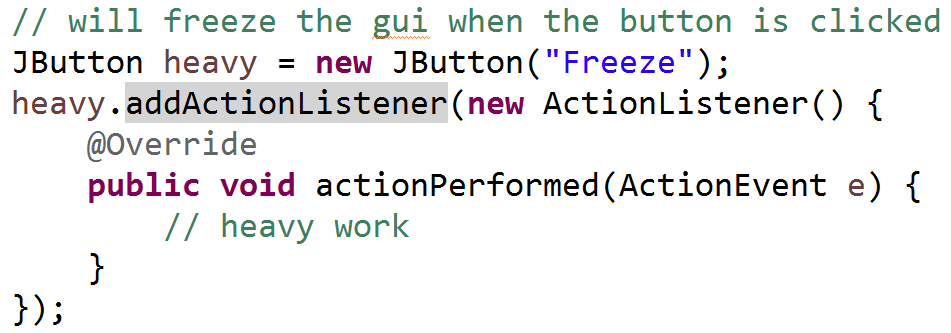
\includegraphics[scale=0.34]{./pics/tut5/mot-par.png}
		\pause
		\begin{itemize}
			\item "'normales"' sequentielles Programm = 1 Prozess mit 1 Thread
			\item paralleles Programm = 1 Prozess mit mehreren Threads
		\end{itemize}
	\end{frame}

	\begin{frame}
		\frametitle{Parallelität in Java}
		\begin{itemize}
			\item in Java zwei Möglichkeiten einen Thread zu erstellen
			\item bereits in Java enthalten:
			\begin{itemize}
				\item Interface \texttt{java.lang.Runnable}
				\item Klasse \texttt{java.lang.Thread}
			\end{itemize}
		\end{itemize}
	\end{frame}

	\begin{frame}
		\frametitle{Parallelität in Java}
		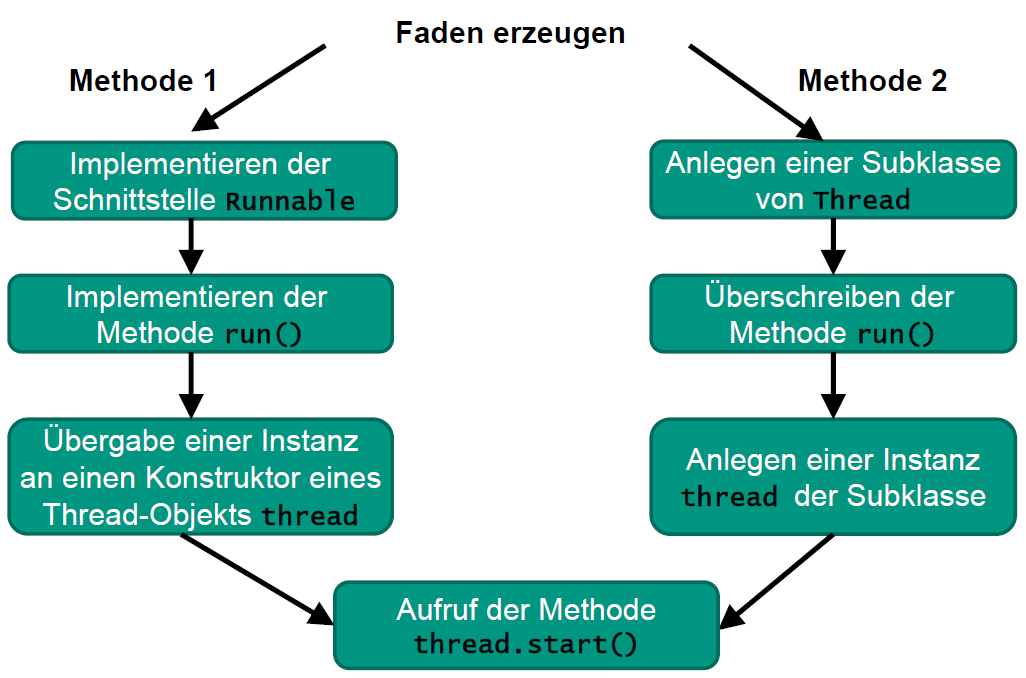
\includegraphics[scale=0.34]{./pics/tut5/crea-thr.png}
	\end{frame}

	\begin{frame}
		\frametitle{Parallelität in Java}
		\centering
		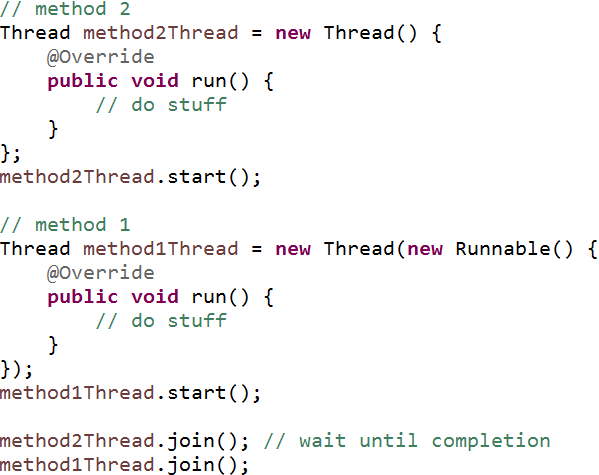
\includegraphics[scale=0.43]{./pics/tut5/crea-thr-java.png}
		\pause
		\begin{alertblock}{Wichtig!}
			\begin{itemize}
				\item immer \texttt{Thread.start()} aufrufen, nicht \texttt{Thread.run()} \pause
				\item \texttt{Thread.run()} würde \texttt{run()} sequenziell aufrufen, \texttt{start()} kehrt direkt zurück, nachdem Thread gestartet wurde
			\end{itemize}
		\end{alertblock}
	\end{frame}

	\begin{frame}
		\frametitle{Synchronisation}
		\begin{itemize}
			\item Problem: Zugriff auf globale Variablen durch mehrere Threads können in beliebiger Reihenfolge passieren
			\item Threads können unterbrochen werden
			\item Folge: ggf. falsche Ergebnisse
		\end{itemize}
		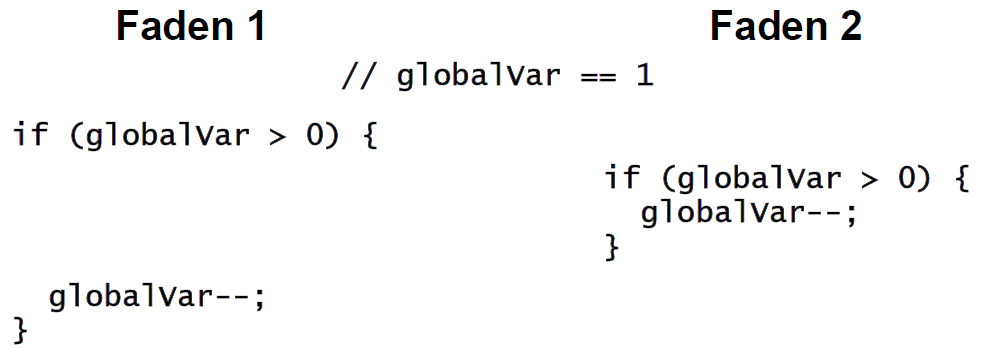
\includegraphics[scale=0.43]{./pics/tut5/par-pro.png}
	\end{frame}

	\begin{frame}{Nicht nur ein theoretisches Problem}
		\centering
		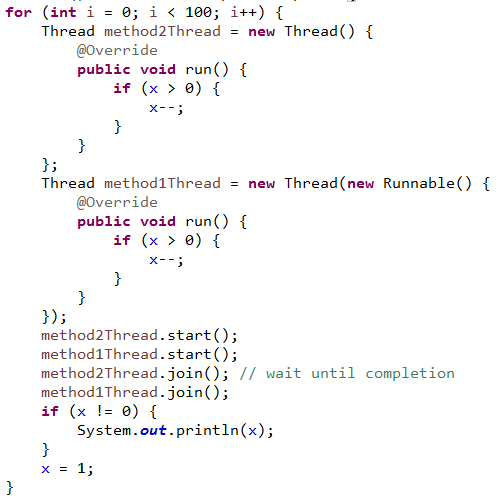
\includegraphics[scale=0.43]{./pics/tut5/synch-ex.png} \pause
		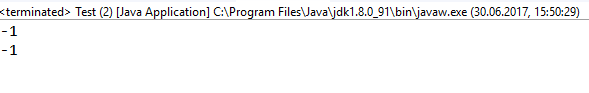
\includegraphics[scale=0.43]{./pics/tut5/synch-ex2.png}
	\end{frame}

	\begin{frame}
		\frametitle{Synchronisation}
		\begin{itemize}
			\item Ziel: Zugriff auf gemeinsam genutzte Daten synchronisieren \pause 
			\begin{itemize}
				\item kritische Abschnitte schützen \pause
				\item Wettlaufsituationen vermeiden
			\end{itemize}
			\begin{block}{Kritischer Abschnitt (critical section)}
				Codeabschnitt, wo Zugriffe auf gemeinsam genutzte Daten stattfinden
			\end{block} \pause
			\begin{block}{Wettlaufsituation (race condition)}
				Verhalten des Programms hängt von der zeitlichen Abfolge der Operationen ab (Wann wird welcher Thread abgebrochen?)
			\end{block} \pause
			\item Idee: Monitor einführen
		\end{itemize}
	\end{frame}

	\begin{frame}
		\frametitle{Monitor}
		\begin{itemize}
			\item Idee: Monitor einführen \pause
			\begin{itemize}
				\item Ziel: Bereich im Code markieren,
				\begin{itemize}
					\item den nur ein Thread gleichzeitig ausführen kann
					\item in dem der Thread nicht unterbrochen werden kann
				\end{itemize}
			\end{itemize} \pause
			\item Schlüsselwort in Java \textcolor{blue}{\texttt{synchronized}} \pause
			\item es wird immer an einem Objekt synchronisiert
			\begin{itemize}
				\item \textcolor{blue}{\texttt{synchronized}}\texttt{(Object o)}\texttt{\{/* zu schützender Code */ \}} \pause
			\end{itemize} 
			\item Thread t kommt an eine mit \textcolor{blue}{\texttt{synchronized}}(\texttt{Object o})\{\dots\} markierte Stelle \pause
			\begin{itemize}
				\item es wird geprüft, ob der Monitor gerade frei ist \pause
				\item ist der Monitor frei, kommt t in den kritischen Abschnitt und der Monitor ist besetzt, bis t den Abschnitt wieder verlässt \pause
				\item ist der Monitor besetzt, wird t blockiert, bis der kritische Abschnitt frei ist
			\end{itemize}
		\end{itemize}
	\end{frame}

	\begin{frame}
		\frametitle{Monitor}
		\texttt{private Object o = new Object();}
		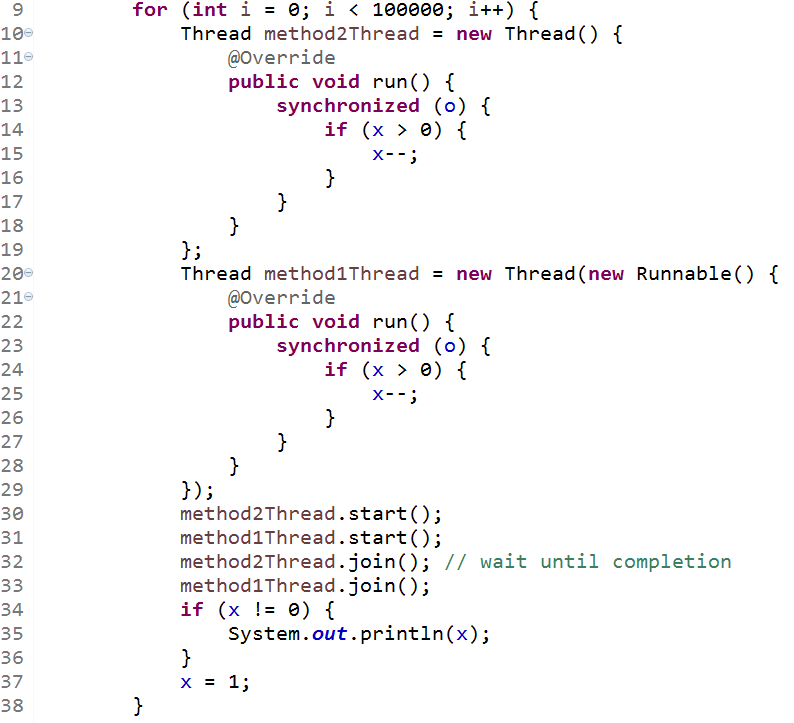
\includegraphics[scale=0.36]{./pics/tut5/synch-ex3.png} \pause
		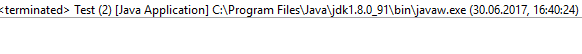
\includegraphics[scale=0.39]{./pics/tut5/synch-ex4.png}
	\end{frame}

	\begin{frame}{Monitor}
		\begin{itemize}
			\item \texttt{synchronized} an Methoden 
			\begin{itemize}
				\item nicht-statische Methode = \texttt{synchronized(this)\{Methoden-Rumpf\}} 
				\item statische Methode = \texttt{synchronized(X.class)\{Methoden-Rumpf\}} 
			\end{itemize}
			\pause 
			\begin{alertblock}{Aber Achtung}
				\begin{itemize}
					\item \texttt{synchronized} killt Parallelität
					\item immer nur ein Thread gleichzeitig im kritischen Abschnitt
					\item also nur dann benutzen wenn wirklich nötig 
					\begin{itemize}
						\item sonst wird alles wieder sequentiell
					\end{itemize} 
					\item außerdem kritische Abschnitte möglichst klein halten
					\begin{itemize}
						\item möglichst wenig Arbeit im Abschnitt machen
					\end{itemize}
				\end{itemize}
			\end{alertblock}

		\end{itemize}
	\end{frame}

	\begin{frame}
		\frametitle{wait() und notify()}
		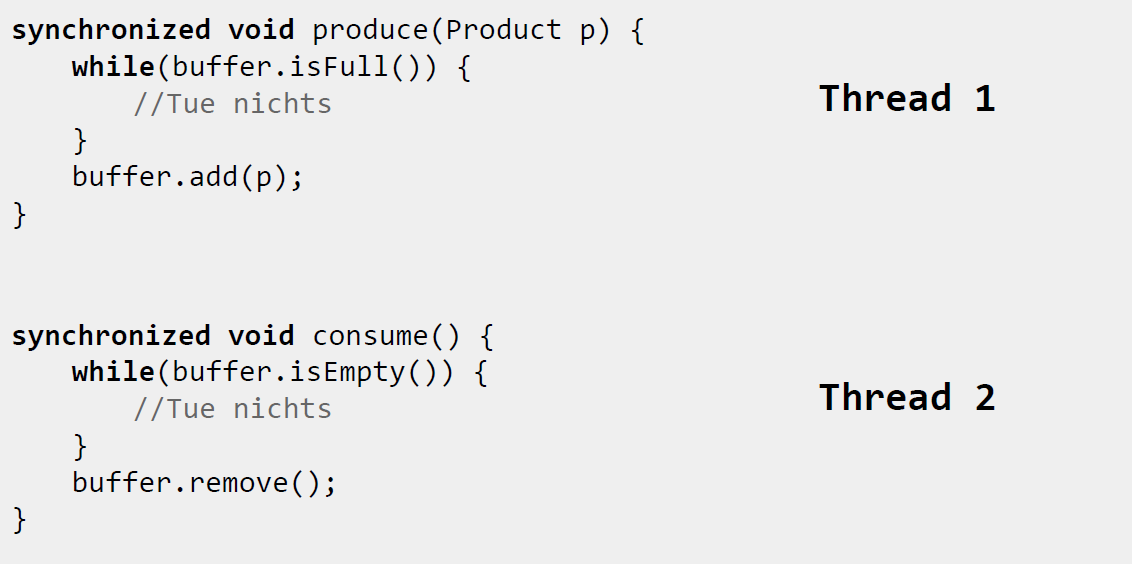
\includegraphics[scale=0.3]{./pics/tut5/cons-prod.png}
		\pause
		\begin{alertblock}{Probleme}
			\begin{itemize}
				\pause
				\item "'busy waiting"' verschwendet Rechenzeit \pause
				\item wartender Produzent blockiert Konsument, der dann nichts konsumieren kann 
			\end{itemize}
		\end{alertblock}
	\end{frame}

	\begin{frame}
		\frametitle{wait() und notify()}
		\begin{itemize}
			\item Idee: brauchen Mechanismus,
			\begin{itemize}
				\item der es erlaubt den Monitor freizugeben, während man auf etwas wartet \pause
				\item der es erlaubt wartende Threads aufzuwecken \pause
			\end{itemize}
			\item in Java: \texttt{wait()} und \texttt{notify()} bzw. \texttt{notifyAll()} \pause
			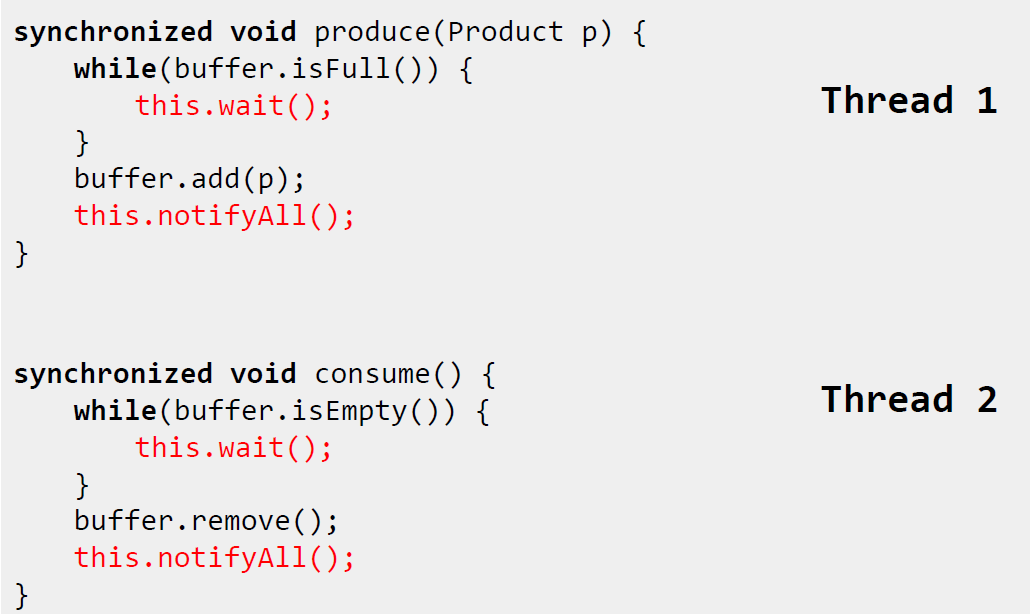
\includegraphics[scale=0.3]{./pics/tut5/cons-prod-sol.png}
		\end{itemize}
	\end{frame}

	\begin{frame}
		\frametitle{wait() und notify()}
		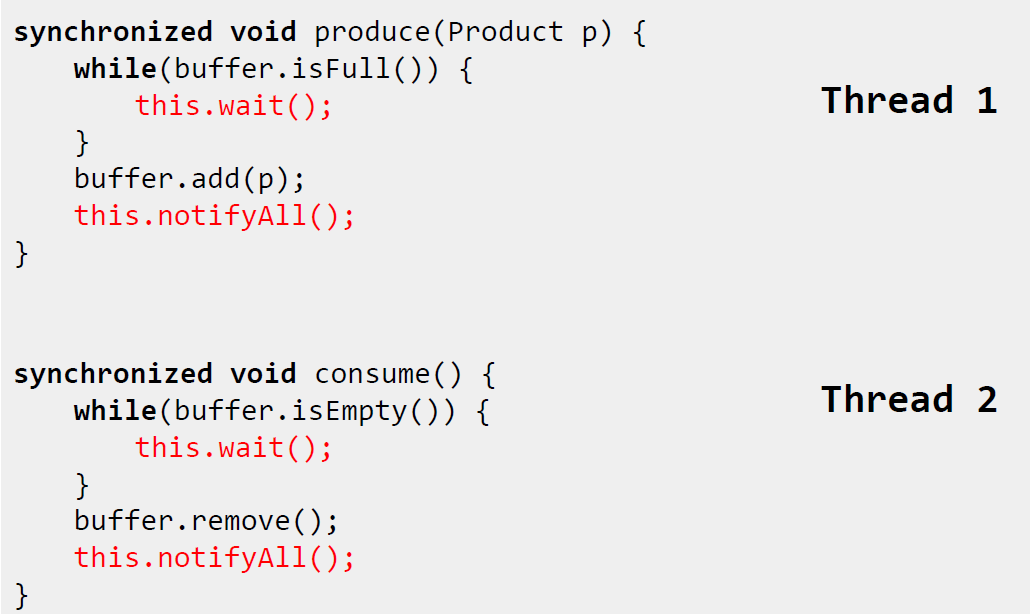
\includegraphics[scale=0.3]{./pics/tut5/cons-prod-sol.png}
		\begin{itemize}
			\item Kann man die while-Schleifen jetzt nicht durch eine if-Abfrage ersetzen? \pause
			\begin{itemize}
				\item Nein, dann würde nach dem Aufwecken nicht nochmal geprüft werden, ob die Bedingung mittlerweile falsch ist.
			\end{itemize}
		\end{itemize}
	\end{frame}

	\begin{frame}
		\frametitle{Verklemmung (deadlock)}
		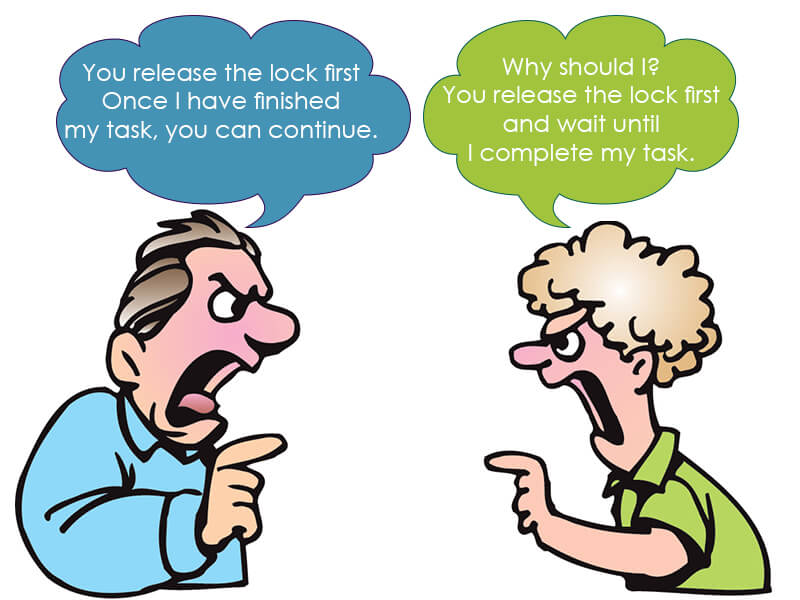
\includegraphics[scale=0.3]{./pics/tut5/deadlock.jpg}
		\pause
		\begin{itemize}
			\item Thread A hält Monitor X und benötigt Monitor Y
			\item Thread B hält Monitor Y und benötigt Monitor X
		\end{itemize}
	\end{frame}

	\begin{frame}
		\frametitle{Deadlock an der PH}
			\centering 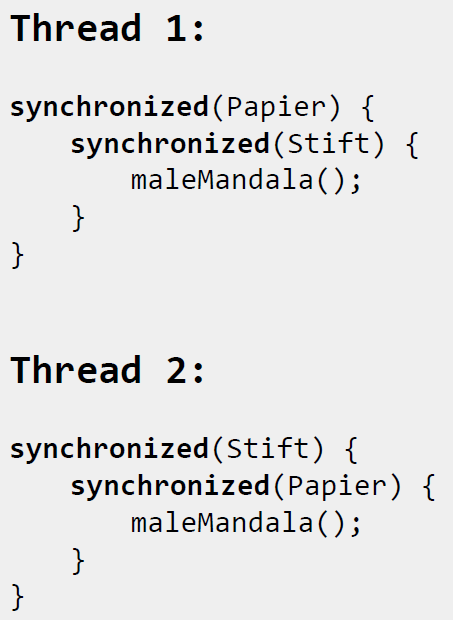
\includegraphics[scale=0.4]{./pics/tut5/deadlock-ex.png}
	\end{frame}

	
	\begin{frame}
		\frametitle{Deadlock an der PH}
		\begin{itemize}
			\item Lösungsansatz: Monitore immer in gleicher Reihenfolge anfordern
		\end{itemize}
		\centering 
		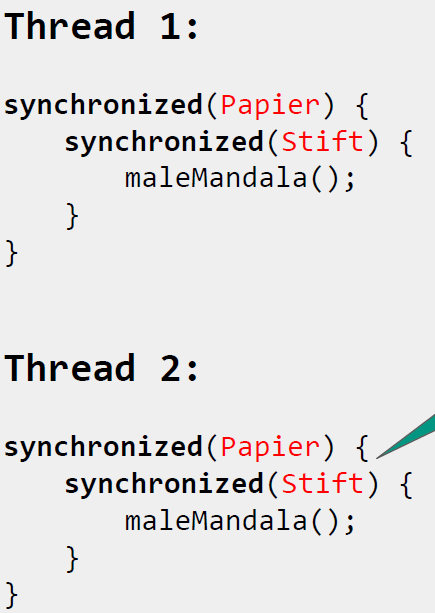
\includegraphics[scale=0.4]{./pics/tut5/deadlock-ex-sol.png}
	\end{frame}

	\begin{frame}{volatile}
		\begin{itemize}
			\item Schlüsselwort \texttt{volatile} an Variablen
			\item Zugriff auf Variablen immer direkt über den Hauptspeicher
			\begin{itemize}
				\item Caches werden umgangen
			\end{itemize}
			\item sorgt dafür, dass alle Threads den gleichen Wert sehen \pause
			\item Compiler darf weniger optimieren
		\end{itemize} \pause
		\begin{exampleblock}{Löst es das folgende Problem?}
			\texttt{i++} ausgeführt von 2 Threads. \texttt{volatile i} ist initial 0. \linebreak Ist i nach der Ausführung immer 2?
		\end{exampleblock} \pause Beispiel-Code \pause
		\begin{itemize}
			\item Nein! 
			\begin{itemize}
				\item \texttt{volatile} kümmert sich nur darum, dass alle Threads die gleiche Sicht auf den Speicher haben
				\item kein Einfluss auf Ausführung
				\item kein Schutz vor race conditions
			\end{itemize}
		\end{itemize}
	\end{frame}
	
	\begin{frame}
		\centering
		\begin{huge}
			Klausuraufgabe SS14
		\end{huge}
	\end{frame}
	
	\begin{frame}
		\frametitle{Parallelität üben}
		\centering \huge \url{https://deadlockempire.github.io/}
	\end{frame}
	
	
	\begin{frame}
		\frametitle{Swing Dispatch Thread}
		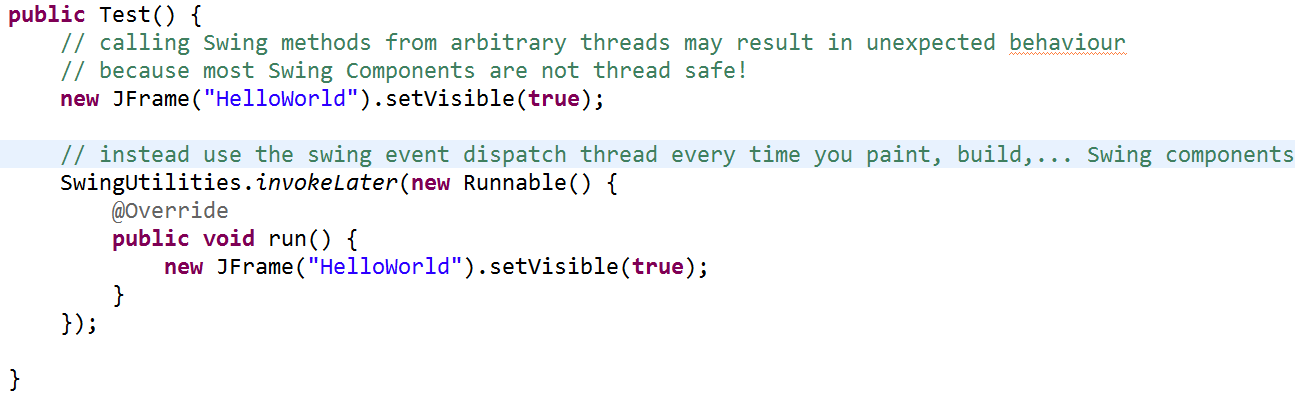
\includegraphics[scale=0.35]{./pics/tut5/edt.png}
		\begin{tiny}
			siehe auch: \url{https://docs.oracle.com/javase/tutorial/uiswing/concurrency/dispatch.html}
		\end{tiny}
	\end{frame}

	\begin{frame}
		\frametitle{Parallelität in GUI nutzen}
		\centering
		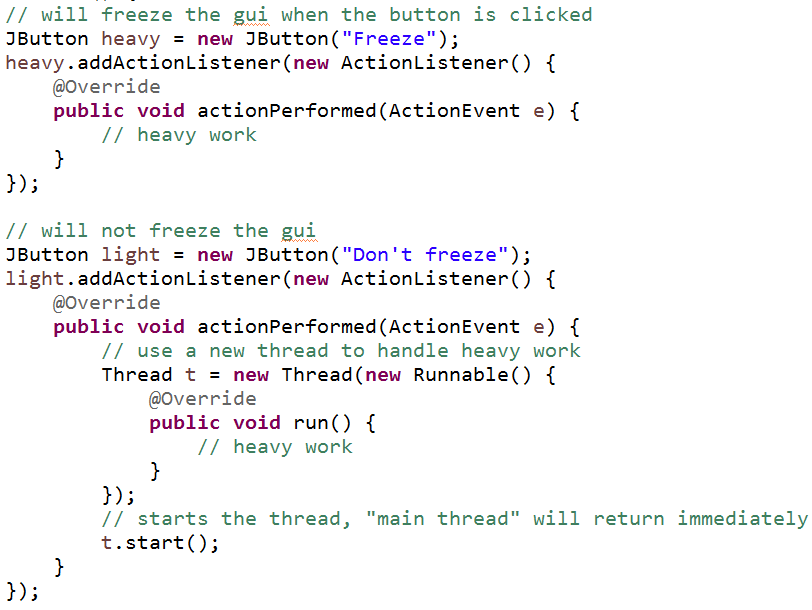
\includegraphics[scale=0.4]{./pics/tut5/extra-thread.png}
	\end{frame}

	\begin{frame}{Wie benutzt man nun Parallelität?}
		\begin{enumerate}
			\item großes Problem
			\item ??? $\rbrace$ Parallelität?
			\item Profit
		\end{enumerate}
	\end{frame}

	\begin{frame}{Wie benutzt man nun Parallelität?}
		\begin{enumerate}
			\item großes Problem in Teilprobleme aufteilen
			\item Teilprobleme durch verschiedene Threads parallel lösen lassen
			\begin{itemize}
				\item Threads manuell verwalten oder Thread-Pool benutzen
			\end{itemize}
			\item Teil-Lösungen zu Gesamt-Lösung zusammensetzen
			\begin{itemize}
				\item auf critical sections/ race conditions achten
			\end{itemize}
			\item Profit = Laufzeit-Reduktion (falls alles richtig gemacht)
		\end{enumerate}
	\end{frame}

\section{Testen}

	\begin{frame}
		\frametitle{Kontrollflussorientiertes Testverfahren (KFO)}
		\begin{itemize}
			\item Ziel: "'sinnvolle"' Testfälle finden
		\end{itemize}
		Vorgehen:
		\begin{enumerate}
			\item gegeben: zu testender Code \pause
			\item Code $\implies$ Zwischensprache
			\begin{itemize}
				\item Sprünge umwandeln
				\item Grundblöcke finden
				\item Grundblöcke prüfen
			\end{itemize}
			\pause
			\item Zwischensprache $\implies$ Kontrollflussgraph \pause
			\item am Kontrollflussgraphen Testfälle finden \pause
			\begin{itemize}
				\item Anweisungsüberdeckung
				\item Zweigüberdeckung 
				\item Pfadüberdeckung
				\item (Bedingungsüberdeckung)
			\end{itemize}
		\end{enumerate}
	\end{frame}

	\begin{frame}[fragile]
		\frametitle{KFO: Code $\rightarrow$ Zwischensprache}
		\begin{itemize}
			\item Sprünge umwandeln
		\end{itemize}
	\centering
			\begin{verbatim}
int a = 9;
int z = 0;
System.out.println("blubb");
while (a == 9) {
  for (int i = 0; i <= b; i++) {
    n++;
  }
  z++;
  if (a == z) {
    a = 8;
  }
}
			\end{verbatim}
	\end{frame}

	\begin{frame}[fragile]{KFO: Code $\rightarrow$ Zwischensprache}
	\begin{itemize}
		\item Sprünge umwandeln (while, for, if, \texttt{x ? a : b},\dots)
		\begin{itemize} 
			\item wie geht das für \texttt{while}, \texttt{if}, \texttt{for}? (Tafel)
			\item Ziel: nur \texttt{if}, \texttt{not}, \texttt{goto} verwenden. Kein \texttt{\{...\}}
		\end{itemize}
	\end{itemize}
	\centering
	\begin{verbatim}
int a = 9;
int z = 0;
System.out.println("blubb");
while (a == 9) { <- hier
  for (int i = 0; i <= b; i++) { <- hier
    n++;
  }
  z++;
  if (a == z) { <- hier
    a = 8;
  }
}
	\end{verbatim}
	\end{frame}

	\begin{frame}[fragile]{Sprünge wurden umgewandelt}
	\begin{verbatim}
01 int a = 9;
02 int z = 0;
03 System.out.println("blubb");
04 if not (a == 9) goto 14;
05 int i = 0;
06 if not (i <= b) goto 10;
07 n++;
08 i++;
09 goto 06;
10 z++;
11 if not (a == z) goto 13;
12 a = 8;
13 goto 04;
14
	\end{verbatim}
	\end{frame}

\begin{frame}{KFO: Code $\rightarrow$ Zwischensprache}
	\begin{itemize}
		\item nächster Schritt: Grundblöcke finden
		\item Code bis \texttt{goto} ist ein Grundblock
	\end{itemize}
\end{frame}

	\begin{frame}[fragile]
\small 
\begin{columns}
	\begin{column}{0.5\textwidth}
		\footnotesize
\begin{verbatim}
01 int a = 9;
02 int z = 0;
03 System.out.println("blubb");
04 if not (a == 9) goto 14;
\end{verbatim}
\begin{verbatim}
05 int i = 0;
06 if not (i <= b) goto 10;
\end{verbatim}
\begin{verbatim}
07 n++;
08 i++;
09 goto 06;
\end{verbatim}
\begin{verbatim}
10 z++;
11 if not (a == z) goto 13;
\end{verbatim}
\begin{verbatim}
12 a = 8;
13 goto 04;
\end{verbatim}
\begin{verbatim}
14
\end{verbatim}
	\end{column}%
	\begin{column}{0.5\textwidth}
		\begin{itemize}
			\item haben erste Grundblöcke gefunden
			\pause
			\item jetzt: Grundblöcke prüfen
			\item \texttt{goto} dürfen nur auf Start eines Blocks verweisen
			\item daher: Blöcke ggf. noch weiter unterteilen
		\end{itemize}
	\end{column}
\end{columns}	
	\end{frame}

	\begin{frame}[fragile]
\small 
\begin{columns}
	\begin{column}{0.5\textwidth}
		\footnotesize
		\begin{verbatim}
		01 int a = 9;
		02 int z = 0;
		03 System.out.println("blubb");
		04 if not (a == 9) goto 14;
		\end{verbatim}
		\begin{verbatim}
		05 int i = 0;
		06 if not (i <= b) goto 10; 
		\end{verbatim}
		\begin{verbatim}
		07 n++;
		08 i++;
		09 goto 06; <-- kaputt!
		\end{verbatim}
		\begin{verbatim}
		10 z++;
		11 if not (a == z) goto 13; <-- kaputt!
		\end{verbatim}
		\begin{verbatim}
		12 a = 8;
		13 goto 04; <-- kaputt!
		\end{verbatim}
		\begin{verbatim}
		14
		\end{verbatim}
	\end{column}%
	\begin{column}{0.5\textwidth}
		\begin{itemize}
			\item haben erste Grundblöcke gefunden
			\item jetzt: Grundblöcke prüfen
			\item \texttt{goto} dürfen nur auf Start eines Blocks verweisen
			\item daher: Blöcke ggf. noch weiter unterteilen
		\end{itemize}
	\end{column}
\end{columns}	
\end{frame}

	\begin{frame}[fragile]
\small 
\begin{columns}
	\begin{column}{0.4\textwidth}
		\scriptsize
		%\fontsize{3mm}{3mm}\selectfont
		\begin{verbatim}
		01 int a = 9;
		02 int z = 0;
		03 System.out.println("blubb");
		\end{verbatim}
		\begin{verbatim}
		04 if not (a == 9) goto 14;
		\end{verbatim}
		\begin{verbatim}
		05 int i = 0;
		\end{verbatim}
		\begin{verbatim}
		06 if not (i <= b) goto 10;
		\end{verbatim}
		\begin{verbatim}
		07 n++;
		08 i++;
		09 goto 06;
		\end{verbatim}
		\begin{verbatim}
		10 z++;
		11 if not (a == z) goto 13;
		\end{verbatim}
		\begin{verbatim}
		12 a = 8;
		\end{verbatim}
		\begin{verbatim}
		13 goto 04;
		\end{verbatim}
		\begin{verbatim}
		14
		\end{verbatim}
	\end{column}%
	\begin{column}{0.6\textwidth}
		\begin{itemize}
			\pause
			\item jetzt sind wir fertig mit den Grundblöcken
			\pause
			\item als nächstes: Graphen hinzeichnen
			\item dazu Start- und Endblock hinzufügen
			\item Blöcke benennen ($n_{start}, n_1, \dots, n_x, n_{stopp}$)
			\item Knoten und Kanten hinzeichnen
		\end{itemize}
	\end{column}
\end{columns}	
\end{frame}


	\begin{frame}
		\centering 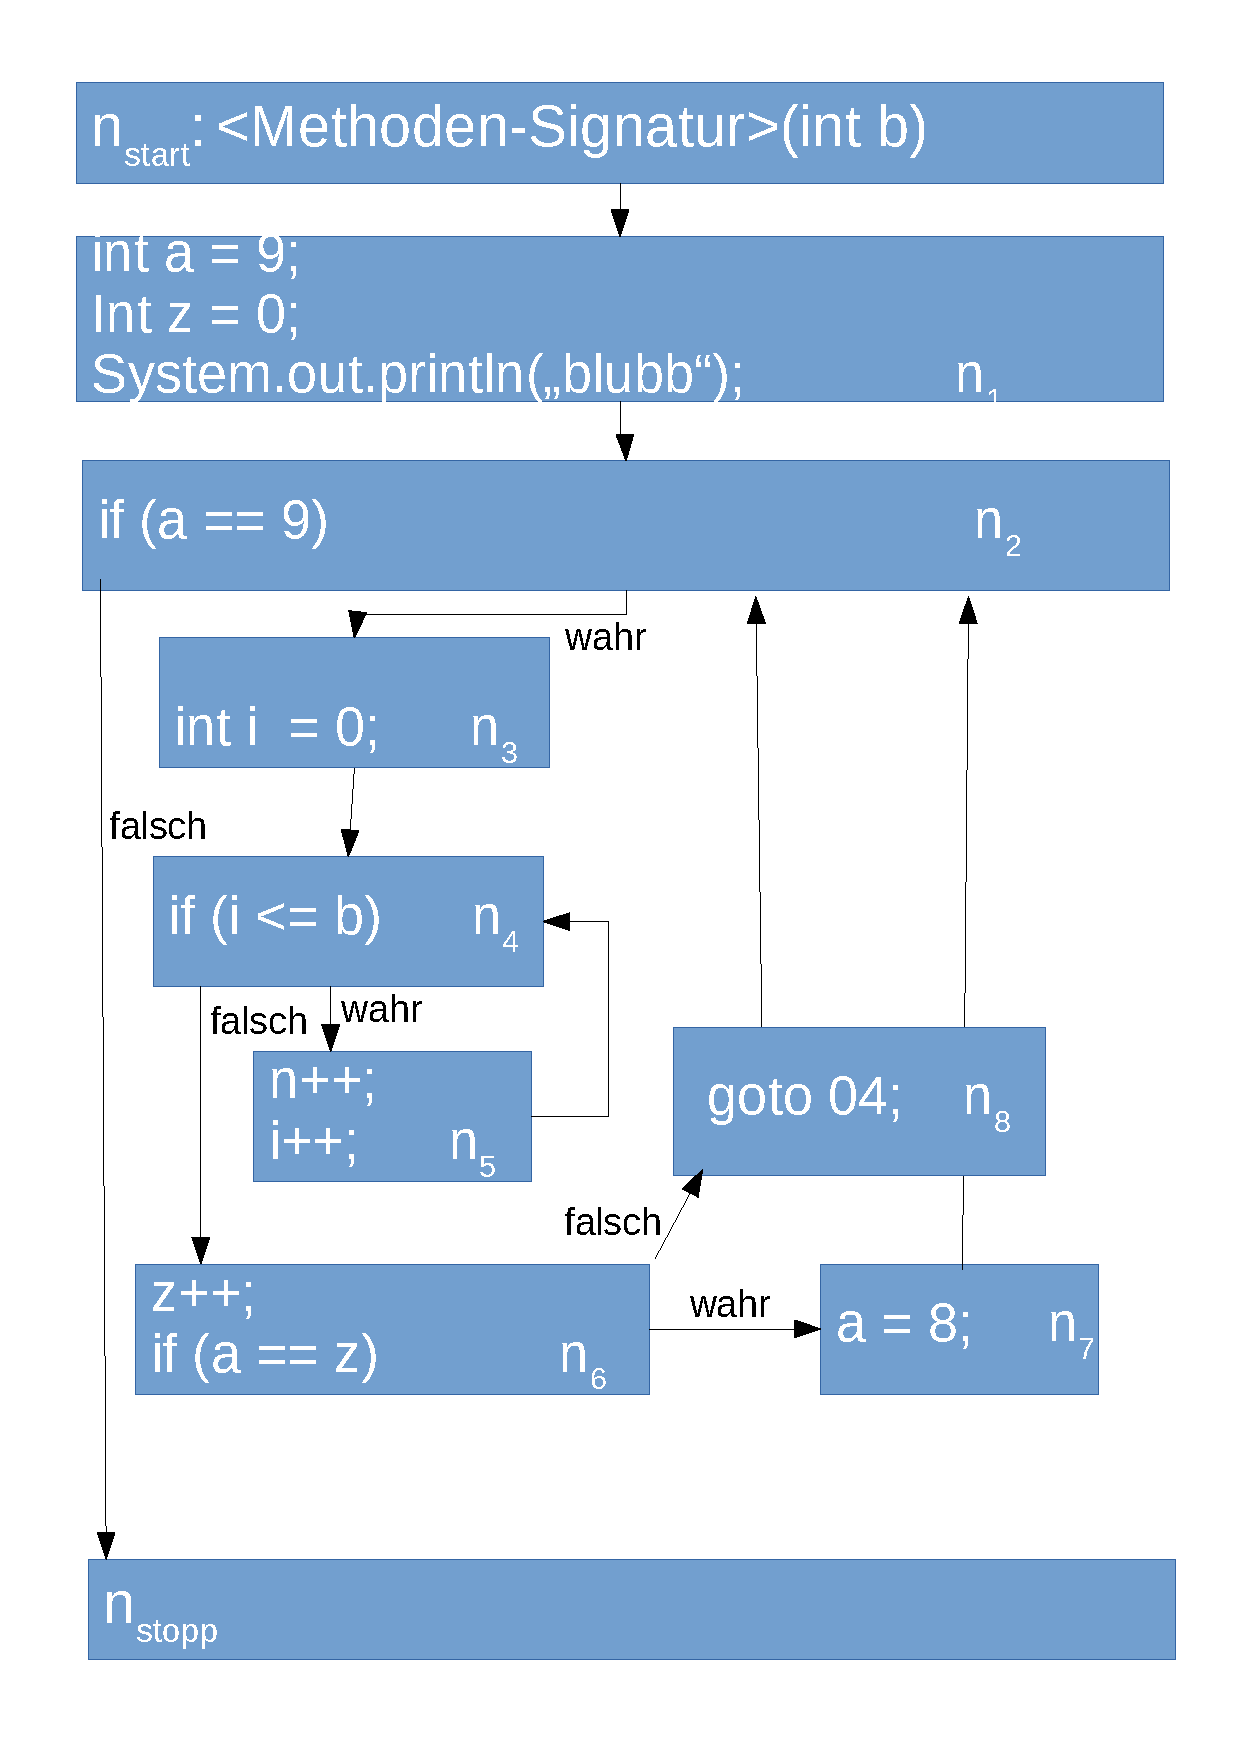
\includegraphics[scale=0.29]{./pics/tut5/kfo.pdf}
	\end{frame}

	\begin{frame}
		\begin{itemize}
			\item goto-Knoten kann man auch weglassen
		\end{itemize}
		\centering 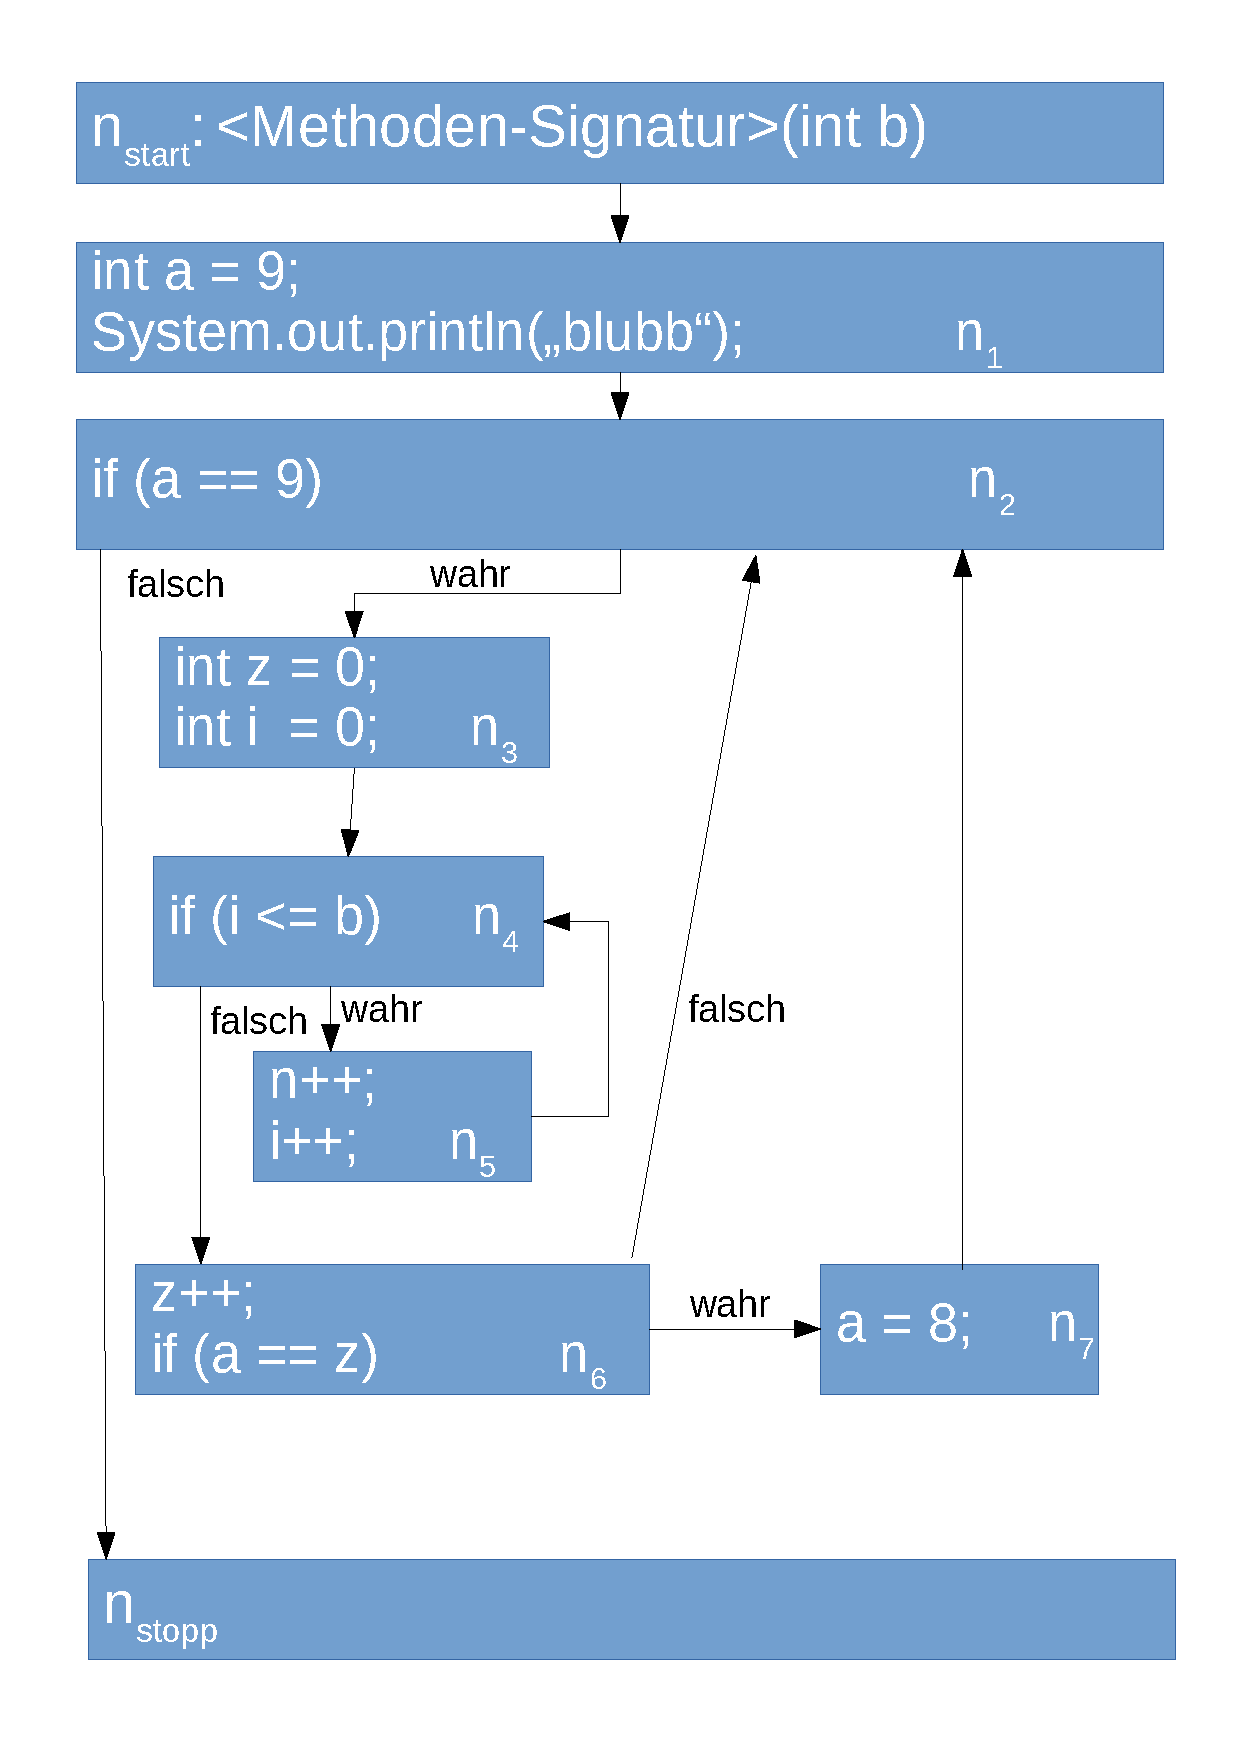
\includegraphics[scale=0.27]{./pics/tut5/kfo-no-goto.pdf}
	\end{frame}

	\begin{frame}
		\frametitle{KFO: Anweisungsüberdeckung}
		\begin{itemize}
			\item wähle Testfälle so, dass jeder Grundblock traversiert wird \pause
			\linebreak $\implies$ Entdeckung nicht erreichbarer Code-Abschnitte \pause
			\item aber: kein ausreichendes Testkriterium
			\begin{itemize}
				\item Schleifen einmal durchlaufen reicht schon
			\end{itemize}
		\end{itemize}
	\end{frame}

	\begin{frame}
		\frametitle{KFO: Zweigüberdeckung}
		\begin{itemize}
			\item wähle Testfälle so, dass jeder Zweig (=Kante) traversiert wird \pause
			\linebreak $\implies$ Entdeckung nicht erreichbarer Kanten \pause
			\item wie bei Anweisungsüberdeckung
			\begin{itemize}
				\item Schleifen werden ggf. nicht ausreichend getestet
			\end{itemize}
		\end{itemize}
	\end{frame}

	\begin{frame}
		\frametitle{KFO: Pfadüberdeckung}
		\begin{itemize}
			\item Finde \textbf{alle} vollständigen, unterschiedlichen Pfade 
			\begin{itemize}
				\item wähle Testfälle so, dass alle gefundenen Pfade durchlaufen werden
			\end{itemize}
			\item vollständiger Pfad = Anfang bei $n_{start}$, Ende bei $n_{stopp}$ \pause
			\item nicht praktikabel, da 
			\begin{itemize}
				\item Schleifen die Anzahl der möglichen Pfade stark erhöhen 
				\begin{itemize}
					\item sogar \enquote{unendlich viele}, wenn Iterationen von Eingabe abhängig\pause
				\end{itemize}
				\item manche Pfade nicht ausführbar sind
				\begin{itemize}
					\item z.B. sich gegenseitig ausschließende Bedingungen
				\end{itemize} 
			\end{itemize}
		\end{itemize}
	\end{frame}

	\begin{frame}{\enquote{Sinnvolle} Testfälle}
		\begin{columns}
			\begin{column}{0.5\textwidth}
				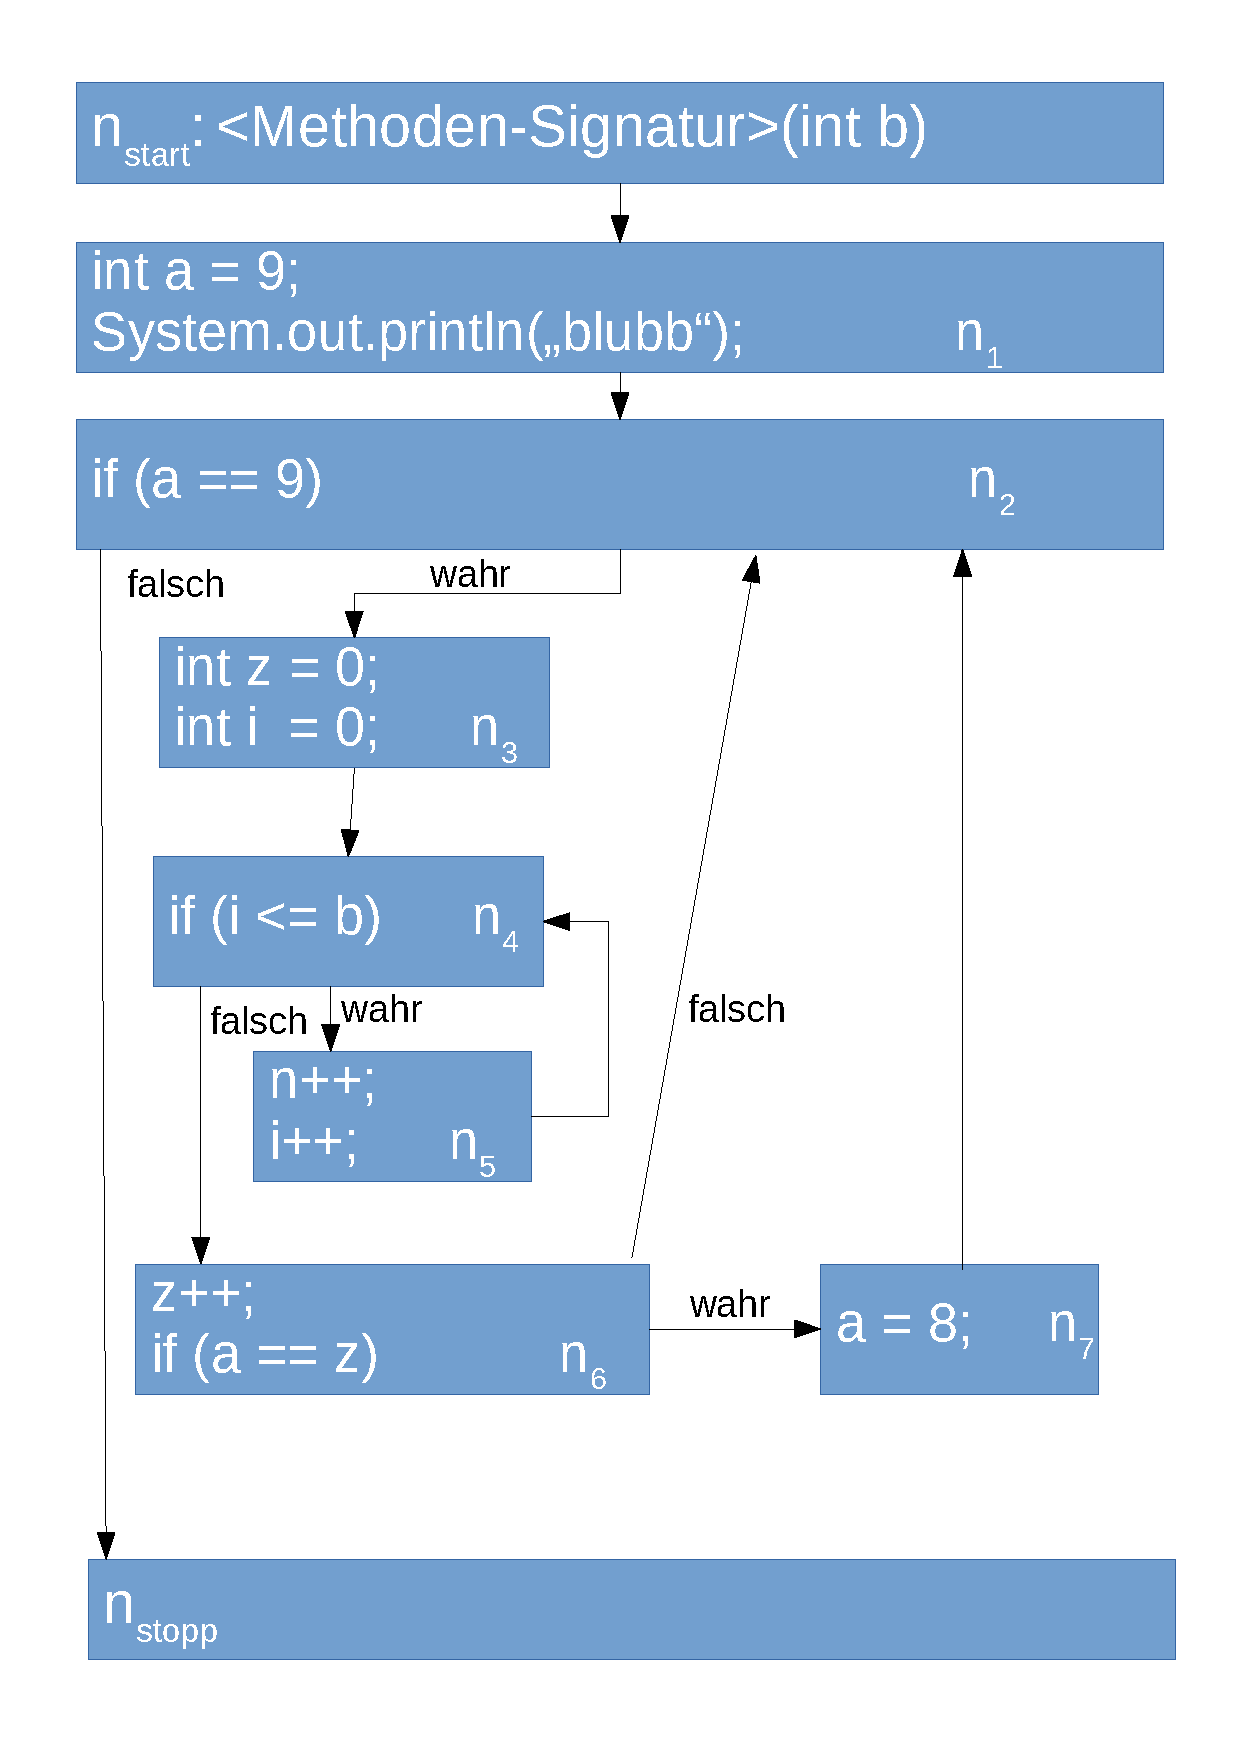
\includegraphics[scale=0.27]{./pics/tut5/kfo-no-goto.pdf}
			\end{column}%
			\begin{column}{0.5\textwidth}
				\begin{itemize}
					\item was ist nun unsere Testfallmenge?			
					\begin{itemize}
						\item = welche \texttt{b} testen?
					\end{itemize}
						\item für Anweisungsüberdeckung?
						\item für Zweigüberdeckung?
				\end{itemize}
			\end{column}
		\end{columns}
	\end{frame}

	\begin{frame}{\enquote{Sinnvolle} Testfälle}
		\begin{columns}
			\begin{column}{0.5\textwidth}
				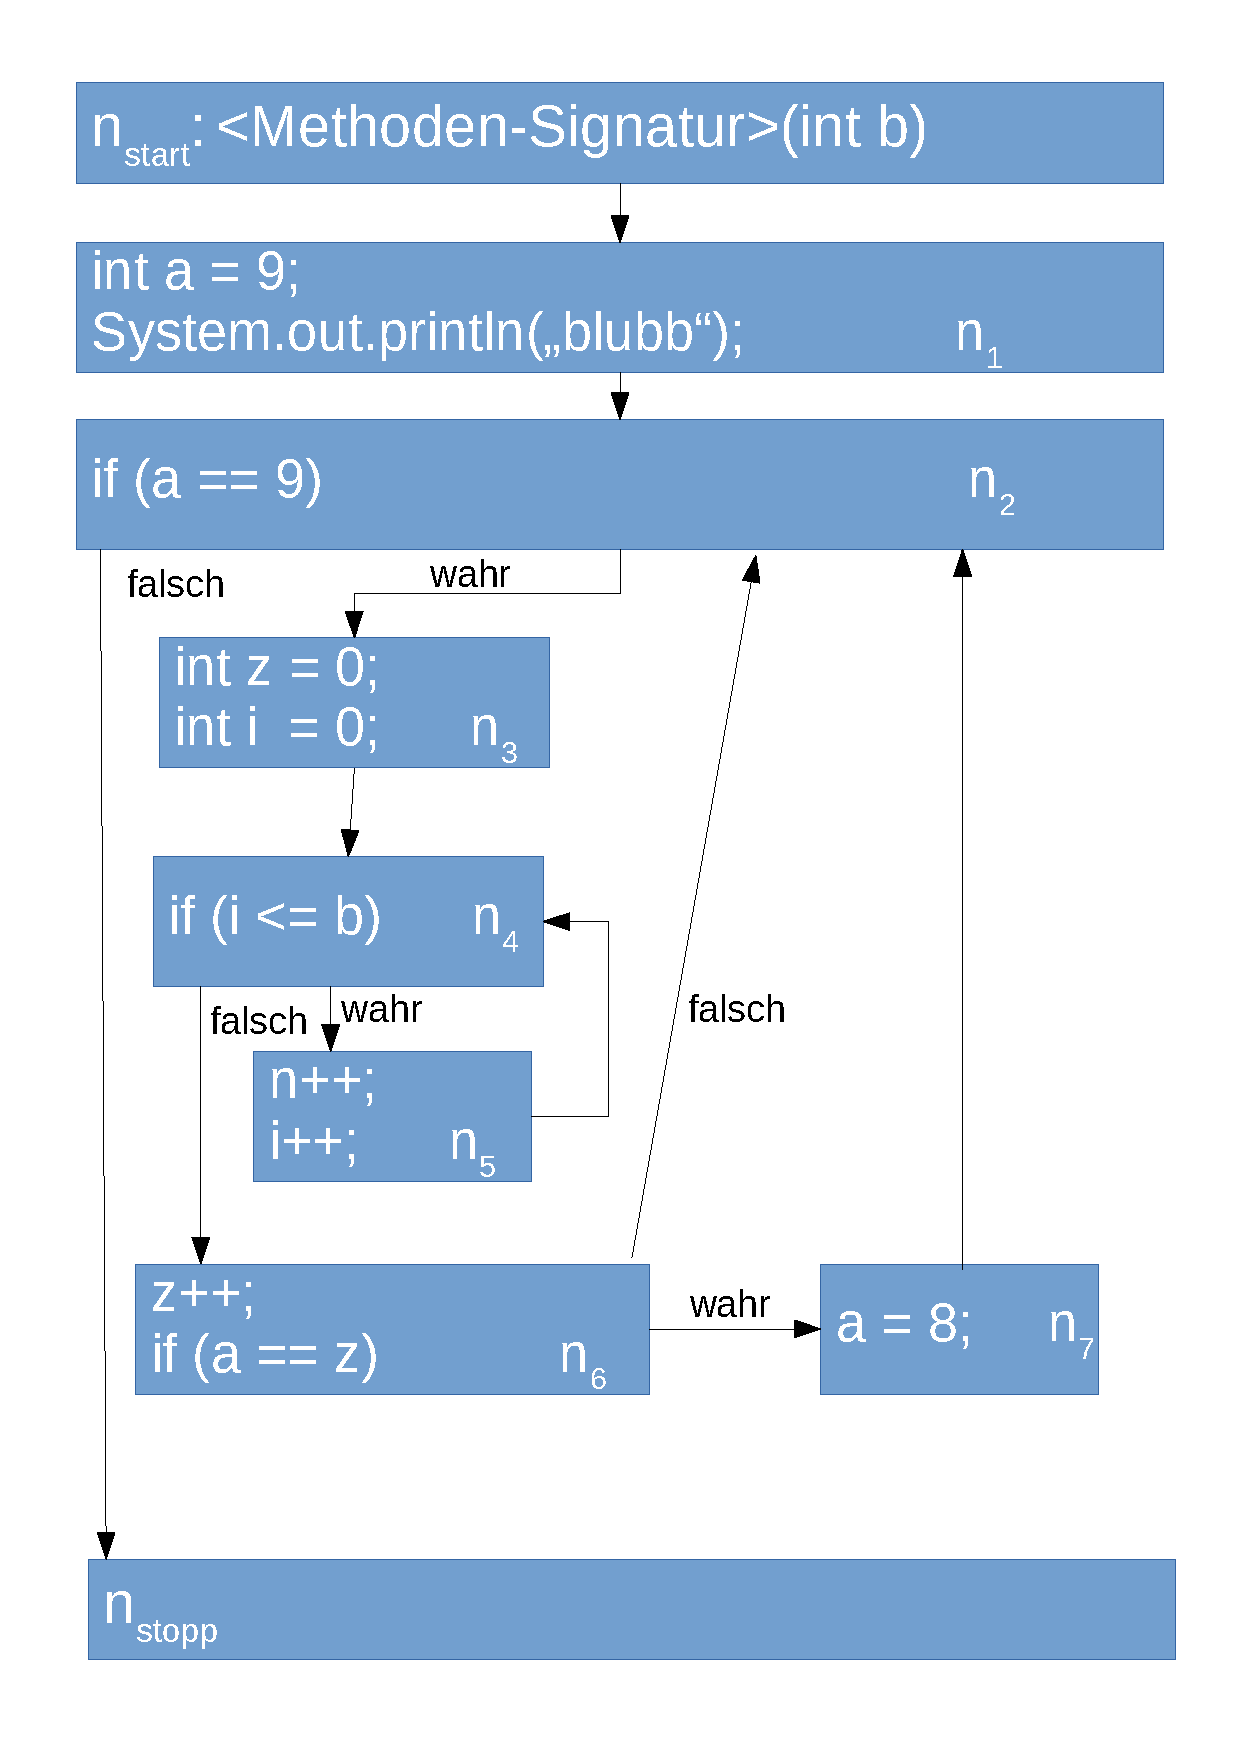
\includegraphics[scale=0.27]{./pics/tut5/kfo-no-goto.pdf}
			\end{column}%
			\begin{column}{0.6\textwidth}
				\begin{itemize}
					\item \texttt{b=0} erfüllt bereits beides
					\item Pfad $(n_{start}, n_1, n_2, n_3, n_4, n_5, n_4, n_6, n_2, \dots, \linebreak n_6, n_7, n_2, n_{stopp})$
					\item i.A. aber mehrere Testfälle nötig
				\end{itemize}
			\end{column}
		\end{columns}
	\end{frame}
		
	\begin{frame}
		\frametitle{Klausuraufgabe SS11}
		\centering 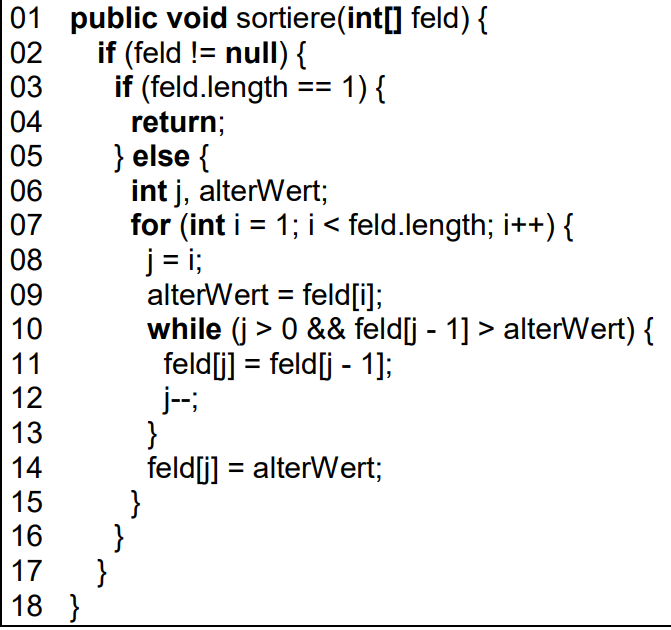
\includegraphics[scale=0.4]{./pics/tut5/exam-task-kfo.png}
		\linebreak
		Erstellen Sie den Kontrollflussgraphen und geben Sie einen Pfad an, der Anweisungsüberdeckung erzielt.
	\end{frame}

	\begin{frame}
		\frametitle{MuLö KFO}
		\centering 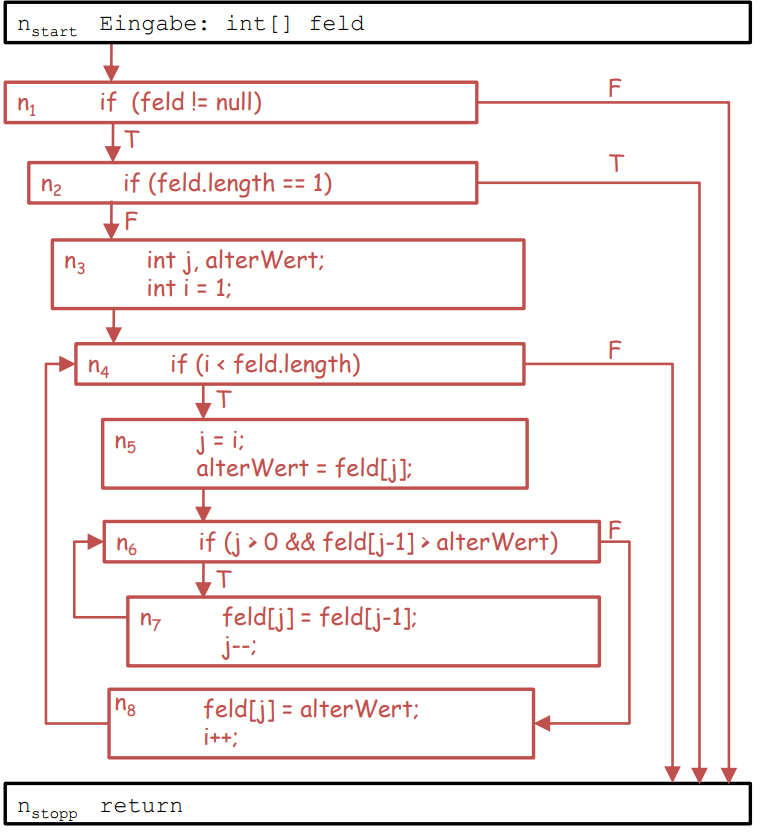
\includegraphics[scale=0.3]{./pics/tut5/exam-task-kfo-sol.png}
		\linebreak \pause
		Pfad: ($n_{start}, n_1, n_2, n_3, n_4, n_5, n_6, n_7, n_6, n_8, n_4, n_{stopp}$) 
	\end{frame}

	\begin{frame}
		\frametitle{Kurzschlussauswertung}
		\begin{alertblock}{Achtung, für ÜBs/Klausur}
			\begin{itemize}
				\item MuLö ist alt, nicht ganz korrekt
				\item Kurzschlussauswertung (\texttt{\&\&} bzw. \texttt{||}) auflösen (in zwei if)
			\end{itemize}
		\end{alertblock}
	\end{frame}


\section{Tipps}
	\subsection{Tipps}
	\begin{frame}
		\frametitle{Tipps - 6. Übungsblatt}

		\begin{exampleblock}{Aufgabe 1: Parallelisierung von HDrize} 
			\begin{itemize}
				\item Berechnung der HDR-Bilder parallelisieren \pause
				\item Thread-Pool spart euch die manuelle Verwaltung der Threads
				\begin{itemize}
					\item \texttt{ExecutorService es = Executors.newFixedThreadPool(amountOfThreads);}
					\item \texttt{es.execute(myRunnable);} (beliebig oft)
					\item \texttt{es.shutdown();}
				\end{itemize} \pause
				\item Tests schreiben
			\end{itemize}
		\end{exampleblock}
		\pause
		\begin{exampleblock}{Aufgabe 2: Parallelisierungswettbewerb}
			\begin{itemize}
				\item Aufgabe 1 verbessern und Laufzeit messen
				\item Teile handschriftlich abgeben
				\begin{itemize}
					\item Laufzeitprofil und Erklärung des Ansatzes
					\item Laufzeitprofil kann man auch ohne weitere Optimierung erstellen ;)
				\end{itemize}
			\end{itemize}
		\end{exampleblock}
	\end{frame}

	\begin{frame}
		\frametitle{Tipps - 6. Übungsblatt}
		\begin{exampleblock}{Aufgabe 3: Kontrollfluss-orientiertes Testen}
			\begin{itemize}
				\item zur Sicherheit Zwischensprache benutzen
				\begin{itemize}
					\item aber auch ok ohne
					\item (hilft aber keine Fehler zu machen)
				\end{itemize}
				\item Achtung: \texttt{\&} vs. \texttt{\&\&}
				\item ansonsten \enquote{Schema F}
			\end{itemize}
		\end{exampleblock}
		\pause
		\begin{exampleblock}{Aufgabe 4: Funktionales Testen}
			\begin{itemize}
				\item Äquivalenzklassen für Parameter finden
				\item auch ungültige und fehlerhafte Eingaben beachten
			\end{itemize}
		\end{exampleblock}
		\pause
		\begin{exampleblock}{Aufgabe 5: Codeinspektion}
			\begin{itemize}
				\item mit Checkliste an eventuellen Problemen Code durchgehen
			\end{itemize}
		\end{exampleblock}

	\end{frame}

	\subsection{Abgabe}
	\begin{frame}
		\frametitle{Denkt dran!}
		\begin{alertblock}{Abgabe}
			\begin{itemize}
				\item Deadline am 17.7. um 12:00
				\item A3-5 und Teile von A2 handschriftlich
				\item auf jeden Fall abgeben, wenn ihr noch Punkte braucht
				\begin{itemize}
					\item aus jeder Aufgabe gute Punkte rauszuholen
				\end{itemize}
			\end{itemize}
		\end{alertblock}
	\end{frame}

	\begin{frame}
		\frametitle{Bis dann! (dann  := 23.07.19)}
		\centering
		
\includegraphics[scale=1.0]{./comics/geek_and_poke_concurrency.jpg}
	\end{frame}

\end{document}